% ===========================================================================
\section{Milestone II: The recombination history}\label{sec:m2}
% ===========================================================================

Before recombination the Universe is filled with a plasma of photons, free electrons and nuclei. Thomson scattering off
the free electrons is so frequent that a photon travels only a tiny distance between collisions, and photons and
baryons move together as a single fluid. When the Universe has cooled enough for electrons to bind into neutral atoms,
the scattering stops: the photons decouple and stream freely towards us as the CMB. This milestone computes the free
electron fraction $X_e(x)$, and from it the optical depth $\tau$ and the visibility function $\gt$, which tells us
where the CMB photons last scattered.

\subsection{Theory}

We define $X_e=n_e/n_H$, where $n_H=(1-Y_p)\rho_b/m_H\propto a^{-3}$ is the number density of hydrogen nuclei, free or
bound, and $Y_p$ is the primordial helium mass fraction. Helium contributes $f_{\rm He}=n_{\rm He}/n_H=Y_p/[4(1-Y_p)]$
nuclei per hydrogen nucleus, so fully ionized hydrogen and helium give $X_e=1+2f_{\rm He}$.

\paragraph*{Saha equilibrium.} At early times the reaction $e^-+p\leftrightarrow{\rm H}+\gamma$ runs much faster than
the expansion and is in chemical equilibrium, $\mu_e+\mu_p=\mu_{\rm H}$ (photons have $\mu_\gamma=0$). The particles are
non-relativistic and non-degenerate, so each species has the Maxwell--Boltzmann density
$n_i=g_i(m_ik_BT/2\pi\hbar^2)^{3/2}e^{(\mu_i-m_ic^2)/k_BT}$. In the ratio $n_en_p/n_{\rm H}$ the chemical potentials
cancel, and the mass difference $m_e+m_p-m_{\rm H}=\epsilon_0/c^2$ leaves the binding energy $\epsilon_0=13.6$\,eV. With
$F=(m_ek_BT_b/2\pi\hbar^2)^{3/2}$ this gives the Saha equation. The same argument applies to the two ionization stages of
helium:
\begin{align}
\frac{n_e x_{\rm H^+}}{1-x_{\rm H^+}} &= F e^{-\epsilon_0/k_BT_b}, \label{eq:saha}\\
\frac{n_e x_{\rm He^+}}{x_{\rm He^0}} &= 4F e^{-\chi_0/k_BT_b},\qquad
\frac{n_e x_{\rm He^{++}}}{x_{\rm He^+}} = F e^{-\chi_1/k_BT_b}.\nonumber
\end{align}
Here $\chi_0=24.59$\,eV and $\chi_1=54.4$\,eV are the helium ionization energies, and the factors $4$ and $1$ are the
ratios of the spin degeneracies. The electron density
$n_e=n_H[x_{\rm H^+}+f_{\rm He}(x_{\rm He^+}+2x_{\rm He^{++}})]$ closes the system. For hydrogen alone,
Eq.~\eqref{eq:saha} is a quadratic in $X_e$.

Equation~\eqref{eq:saha} explains why recombination happens so late. Writing $n_e=X_en_H$ and $n_H\propto\eta_bn_\gamma$,
with $\eta_b\approx6\times10^{-10}$ baryons per photon, the right-hand side divided by $n_H$ is of order
$\eta_b^{-1}(k_BT/m_ec^2)^{3/2}e^{-\epsilon_0/k_BT}$. The huge factor $\eta_b^{-1}$ keeps hydrogen ionized until the
exponential has become very small, i.e.\ until $\epsilon_0/k_BT\approx40$--$50$. Physically, there are so many photons
per atom that even the far Wien tail of the Planck spectrum, above $13.6$\,eV, contains enough photons to ionize every
atom that forms.

\paragraph*{Peebles equation.} As $X_e$ drops, the rates fall below the expansion rate and equilibrium can no longer
be maintained. Recombination is moreover not a single-step process. A direct recombination to the ground state emits a
photon above $13.6$\,eV, which is immediately absorbed by a neighbouring atom and ionizes it again; such recombinations
achieve nothing. Recombination to an excited state cascades down to $n=2$. From $2p$ the atom emits a Lyman-$\alpha$
photon, but the Universe is extremely optically thick to Lyman-$\alpha$, so the photon is reabsorbed and the atom is
re-excited. Only two routes lead permanently to the ground state:
\begin{itemize}
\item the slow two-photon decay $2s\to1s$, with rate $\Lambda_{2s\to1s}=8.227\,{\rm s}^{-1}$;
\item the redshifting of a Lyman-$\alpha$ photon out of the line by the expansion, with rate $\Lambda_\alpha$.
\end{itemize}
Meanwhile the $n=2$ state, bound by only $\epsilon_0/4=3.4$\,eV, is easily photoionized again. Peebles' effective
three-level atom~\cite{Peebles1968} captures this physics:
\begin{equation}
\frac{\dd X_e}{\dd x} = \frac{C_r(T_b)}{H}\Big[\beta(T_b)(1-X_e) - n_H\alpha^{(2)}(T_b)X_e^2\Big].
\label{eq:peebles}
\end{equation}
The terms are as follows:
\begin{itemize}
\item The second term in the bracket is recombination. Its rate per hydrogen atom is $n_e\alpha^{(2)}$, where
      $\alpha^{(2)}$ is the case-B recombination coefficient. It counts only captures to $n\ge2$, the ones that can
      eventually lead to a neutral atom.
\item The first term is photoionization. Its rate $\beta$ follows from $\alpha^{(2)}$ by detailed balance,
      $\beta=\alpha^{(2)}Fe^{-\epsilon_0/k_BT_b}$, so that the bracket vanishes in Saha equilibrium. The rate out of
      $n=2$ is $\beta^{(2)}=\beta e^{3\epsilon_0/4k_BT_b}$.
\item The factor
\begin{equation}
C_r = \frac{\Lambda_{2s\to1s}+\Lambda_\alpha}{\Lambda_{2s\to1s}+\Lambda_\alpha+\beta^{(2)}},\quad
\Lambda_\alpha = \frac{H(3\epsilon_0)^3}{(8\pi)^2(\hbar c)^3 n_{1s}},
\end{equation}
      with $n_{1s}=(1-X_e)n_H$, is the probability that an atom in $n=2$ reaches the ground state before it is ionized
      again.
\end{itemize}
Early on $\beta^{(2)}\gg\Lambda$'s and $C_r\ll1$: this bottleneck makes recombination slower than in equilibrium. Late
on, the recombination rate $n_e\alpha^{(2)}$ drops below $H$ because both $n_e$ and $\alpha^{(2)}$ decrease. The few
remaining electrons can no longer find a proton within a Hubble time, and $X_e$ freezes out at a finite value. The rate
coefficients we use are those of Callin~\cite{Callin2006}.

\paragraph*{Baryon temperature.} The gas is kept at the photon temperature by Compton scattering of the abundant CMB
photons off the free electrons. A non-relativistic gas expanding adiabatically would instead cool as
$T_b\propto a^{-2}$, faster than $T_\gamma\propto a^{-1}$. The two effects combine to
\begin{equation}
\frac{\dd T_b}{\dd x} = -2T_b + \frac{8\sigma_Ta_RT_\gamma^4}{3m_ecH}\frac{X_e}{1+f_{\rm He}+X_e}(T_\gamma-T_b),
\end{equation}
where the second term is the Compton heating rate in units of $H$; the fraction counts the energy transferred per
particle in the gas. This rate is $\sim10^6$ at recombination, so $T_b=T_\gamma$ until the residual electrons become too
few. The baryon temperature enters Eq.~\eqref{eq:peebles} and matters mainly for the freeze-out value of $X_e$.

\paragraph*{Reionization.} The intergalactic medium is ionized today. Ultraviolet radiation from the first stars and
galaxies reionized hydrogen (and helium once) at $z\sim6$--$10$, and quasars reionized the second helium electron at
$z\sim3$. We do not model these sources. Instead we use the phenomenological CAMB/CLASS parametrization~\cite{Lewis2008}:
\begin{align}
X_e &= X_e^{\rm rec} + (1+f_{\rm He}-X_e^{\rm rec})\frac{1+\tanh u}{2} \nonumber\\
    &\quad + f_{\rm He}\frac{1+\tanh u_{\rm He}}{2},
\end{align}
with $u=(y_{\rm re}-y)/\Delta y$, $y=(1+z)^{3/2}$, $\Delta y=\tfrac32(1+z_{\rm re})^{1/2}\Delta z$, and
$u_{\rm He}=(z_{\rm He}-z)/\Delta z_{\rm He}$. The variable $y$ is proportional to the cosmic time during MD, so the
transition is symmetric in time. Hydrogen and the first helium electron are reionized at $z_{\rm re}=8$, and the second
helium electron at $z_{\rm He}=3.5$.

\paragraph*{Optical depth and visibility.} A photon travelling through a gas of free electrons scatters at the rate
$n_e\sigma_Tc$, where $\sigma_T$ is the Thomson cross section. The probability that a photon emitted at $x$ reaches
us without scattering is $e^{-\tau(x)}$, where the optical depth $\tau(x)=\int_x^0 n_e\sigma_Tc\,\dd t$ obeys
\begin{equation}
\tau'(x) = -\frac{c\,n_e\sigma_T}{H},\qquad \gt(x) = -\tau'e^{-\tau}.
\end{equation}
$|\tau'|$ is the number of scatterings per Hubble time. The visibility function $\gt$ is the probability density, per
unit $x$, that a photon observed today scattered for the last time at $x$, and $\int\gt\,\dd x=1$. It peaks where the
falling scattering rate and the growing transparency balance.

\paragraph*{The sound horizon and the drag epoch.} Before decoupling, photons and baryons form one fluid. The photons
provide the pressure, $P=\rho_\gamma c^2/3$, while both components provide the inertia. The sound speed is
$c_s^2=\delta P/\delta\rho=\tfrac{c^2}{3}(1+R_b)^{-1}$, with $R_b=3\rho_b/4\rho_\gamma$. Following
Ref.~\cite{Callin2006} we use the inverse, $R=1/R_b=4\Om_{\gamma0}/(3\Om_{b0}a)$, so
\begin{equation}
r_s(x) = \int_{-\infty}^x\frac{c_s}{\Hp}\dd x',\quad c_s=c\sqrt{\frac{R}{3(1+R)}}.
\end{equation}
$r_s$ is the comoving distance a sound wave travels before $x$. It is the length scale imprinted in both the CMB
peaks and the clustering of galaxies, the baryon acoustic oscillation (BAO) scale. The photons decouple at $\tau=1$.
The baryons are released later. There are $\sim10^9$ photons per baryon, so each baryon keeps being pushed by
scattering photons after a typical photon has stopped scattering. The rate at which the photons transfer momentum to
the baryons is $|\tau'|$ times the ratio of photon to baryon momentum density, $|\tau'|/R_b=|\tau'|R$. The drag epoch is
where the drag optical depth $\tau_d(x)=-\int_x^0\tau'R\,\dd x'$ reaches 1. Since $R>1$ at recombination, it comes
after decoupling.

\subsection{Implementation and tests}

\texttt{RecombinationHistory} solves on 40\,000 points in $x\in[-20,0]$. We use Saha for hydrogen and helium while the
hydrogen ionization fraction is above $0.99$, solving the coupled Saha system by root finding in $\ln n_e$. After that,
$x_{\rm H^+}$ follows the Peebles equation~\eqref{eq:peebles} together with $T_b$. Helium stays in Saha equilibrium, given
the electron density. The coupled $(X_e,T_b)$ system is stiff, because the Compton rate is $\sim10^6H$, so we use the
implicit multistep BDF method of GSL. $X_e$ is splined in $\ln X_e$, which varies over many decades. We integrate
$\tau$ backwards from $\tau(0)=0$, and take $\tau'$ analytically from $n_e$. The code can switch off helium,
reionization, $T_b$ evolution and the Peebles stage (pure Saha), and includes the RECFAST fudge factor $1.14$ on
$\alpha^{(2)}$ as an option~\cite{Seager1999}.

Tests (Figs.~\ref{fig:Xe}--\ref{fig:g}) include:
\begin{itemize}
\item $X_e=1+2f_{\rm He}=1.162$ before helium recombination and $1+f_{\rm He}$ on the He$^+$ plateau.
\item With $Y_p=0$ the full helium solver reproduces the hydrogen-only code exactly (maximum relative difference 0).
\item $\int\gt\,\dd x=1$ to machine precision.
\item $\tau'$, $\tau''$, $\gt'$ and $\gt''$ agree with finite differences of the splines.
\item $r_s$ agrees with an independent quadrature.
\item $T_b=T_\gamma$ at high $z$ and $T_b\propto a^{-2}$ at low $z$.
\item The optical depth to reionization agrees with the analytic estimate for instantaneous reionization in a
      matter+$\Lambda$ background (see below).
\end{itemize}

\subsection{Results}

\begin{figure*}
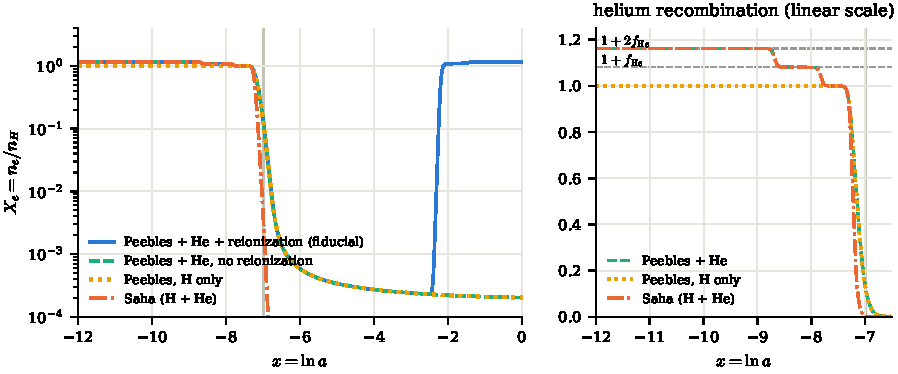
\includegraphics[width=\textwidth]{m2_Xe}
\caption{Free electron fraction. \emph{Left:} the fiducial model (Peebles hydrogen, Saha helium and reionization),
the same without reionization, the hydrogen-only Peebles solution, and the Saha solution for H and He. The vertical
line marks the last-scattering surface ($\tau=1$). \emph{Right:} the same on a linear scale, showing the two helium
recombinations at $z\approx6000$ and $z\approx2500$ before hydrogen recombination.}
\label{fig:Xe}
\end{figure*}

\paragraph*{Helium and hydrogen recombination.} Figure~\ref{fig:Xe} shows the free electron fraction. Helium
recombines first, in two steps, because its electrons are more tightly bound:
\begin{itemize}
\item He$^{++}\to$He$^+$ (54.4\,eV) at $z\approx6000$, the drop from $1.162$ to $1.081$;
\item He$^+\to$He (24.6\,eV) at $z\approx2500$, the drop from $1.081$ to $1$.
\end{itemize}
Both happen when $\chi/k_BT\approx40$, the same ``$\eta_b^{-1}$ delay'' as for hydrogen. Helium is fully neutral
long before hydrogen recombination starts. It therefore has no direct effect on the last-scattering surface; it
matters only by removing electrons at $z\gtrsim2000$, which affects the diffusion damping of small-scale anisotropies.
The hydrogen-only run gives the same numbers as the run with helium to better than $10^{-8}$ (both runs use the same
$n_H$).

Hydrogen recombines between $z\approx1500$ and $z\approx900$. With the Peebles equation $X_e=0.5$ at $z=1273$
($T=3475$\,K, $k_BT=0.30$\,eV), so indeed $\epsilon_0/k_BT\approx45$. Table~\ref{tab:m2} lists the key times. Here we
switch reionization off, so that $\tau$ measures the recombination surface alone.

\paragraph*{Saha versus Peebles.} The Saha approximation recombines far too early and too fast: $X_e=0.5$ at $z=1369$,
decoupling at $z=1291$, and $r_s$ is $11\%$ smaller. Saha assumes that the reactions are instantaneous. In reality the
$n=2$ bottleneck limits the net recombination rate: at $z=1200$ we find $C_r\approx0.007$, so most atoms that
reach $n=2$ are ionized again before they reach the ground state. Recombination therefore falls behind equilibrium.
The difference grows with time. In Saha equilibrium $X_e$ drops exponentially and reaches the numerical floor of
$10^{-30}$ in our code. In the Peebles solution the recombination rate per electron, $n_H\alpha^{(2)}X_e$, falls below
$H$ at $z\approx400$, and the residual ionization freezes at $X_e=2.0\times10^{-4}$ today. These residual electrons keep
$T_b$ coupled to $T_\gamma$ until $z\approx500$ and are important for the formation of the first molecules.

The RECFAST fudge factor 1.14 on $\alpha^{(2)}$ mimics the effect of a full multi-level atom. It speeds up recombination
slightly: $z_*$ changes by $+0.8$, $r_s$ by $0.05\%$, and the freeze-out value is lowered to $1.8\times10^{-4}$. These
small changes nevertheless matter at the precision of Planck.

\begin{table}
\caption{Recombination and decoupling without reionization for the Peebles (with Saha helium) and pure Saha
solutions. Times are cosmic times; $r_s$ is the comoving sound horizon.}
\label{tab:m2}
\begin{ruledtabular}
\begin{tabular}{lcc}
 & Peebles & Saha \\
\hline
$X_e=0.5$: $z$ & $1272.9$ & $1369.1$ \\
Recombination, $X_e=0.1$: $x$ & $-6.9696$ & $-7.1335$ \\
\phantom{Recombination,} $z$ & $1062.8$ & $1252.2$ \\
\phantom{Recombination,} $t$ [kyr] & $387.9$ & $294.1$ \\
Decoupling, $\tau=1$: $x$ & $-6.9943$ & $-7.1640$ \\
\phantom{Decoupling,} $z$ & $1089.4$ & $1291.0$ \\
\phantom{Decoupling,} $t$ [kyr] & $372.1$ & $279.2$ \\
Peak of $\gt$: $z$ & $1085.2$ & $1286.1$ \\
$r_s(\tau=1)$ [Mpc] & $144.46$ & $128.95$ \\
Drag epoch: $z_d$ & $1059.8$ & $1259.5$ \\
$r_s(z_d)$ [Mpc] & $147.08$ & $131.13$ \\
$X_e$ today & $2.03\times10^{-4}$ & $\to0$ \\
\end{tabular}
\end{ruledtabular}
\end{table}

\paragraph*{Decoupling.} The photons decouple ($\tau=1$) at $z=1090$, when the Universe is $372\,000$ years old and
$T=2970$\,K. At that moment $X_e=0.13$: decoupling does not require the gas to be fully neutral, only that the
scattering rate drops below the expansion rate. Indeed $|\tau'|=13$ at $\tau=1$, so a photon still scatters a few
more times per Hubble time, but $X_e$ is dropping so fast that these scatterings stop within $\Delta x\sim0.1$. The
comoving mean free path at that time is $16\Mpc$, compared with the horizon $\eta_*=280\Mpc$. Decoupling is at lower
$z$ than $X_e=0.5$ and higher $z$ than $X_e=0.1$ ($z=1063$). Within a few percent, ``recombination'' and ``last
scattering'' are the same event for the purpose of the CMB.

\begin{figure}
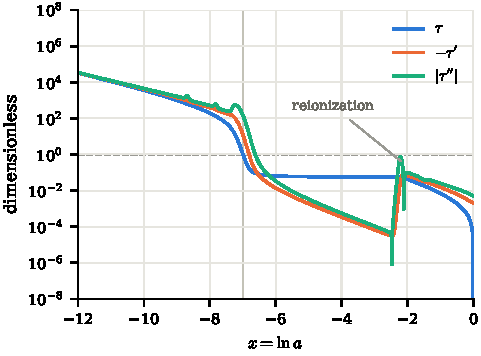
\includegraphics[width=\columnwidth]{m2_tau}
\caption{Optical depth $\tau$ and its derivatives for the fiducial model. $\tau$ drops by many orders of magnitude
during recombination. Reionization gives the shoulder at $x\approx-2$ and the total $\tau_{\rm reion}=0.058$.}
\label{fig:tau}
\end{figure}

\begin{figure*}
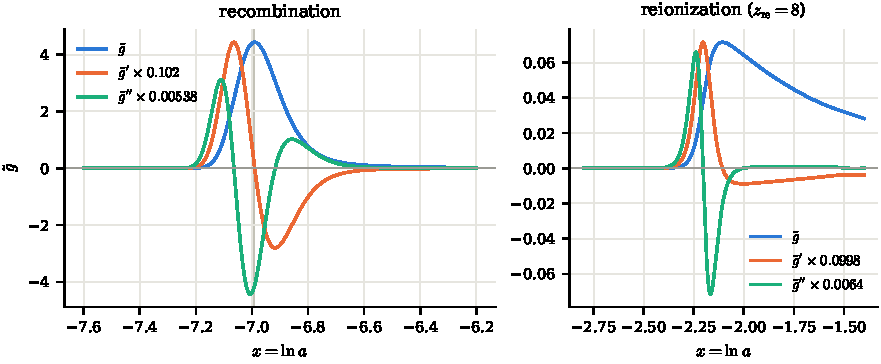
\includegraphics[width=\textwidth]{m2_g}
\caption{Visibility function $\gt$ and its first two derivatives (rescaled to the same amplitude) around recombination
(\emph{left}) and reionization (\emph{right}). The vertical line in the left panel marks $\tau=1$.}
\label{fig:g}
\end{figure*}

\paragraph*{Optical depth and visibility.} Figure~\ref{fig:tau} shows the optical depth. Before recombination
$\tau\propto$ a high power of $a^{-1}$, because $n_e\propto a^{-3}$ and $H\propto a^{-2}$ in RD. Across recombination
$|\tau'|$ drops by more than three orders of magnitude, so the Universe goes from opaque to transparent within a
small fraction of a Hubble time. Figure~\ref{fig:g} shows the visibility function. It is sharply peaked around
$x\approx-7$, with a full width at half maximum of $\Delta x\approx0.18$ ($\Delta z\approx200$). This corresponds to
a comoving thickness of $\approx39\Mpc$, about a quarter of the sound horizon. About two thirds of the CMB photons last
scattered between $z=1000$ and $z=1200$. The finite thickness of the last-scattering surface has two observable
consequences: anisotropies on scales smaller than its thickness are washed out, and polarization is generated only
within it (Sec.~\ref{sec:m3}). The derivatives $\gt'$ and $\gt''$, which appear in the source function, are smooth and
well resolved by our grid.

\paragraph*{Sound horizon and drag epoch.} At decoupling $R_b=0.62$, so the sound speed is $c_s=0.45c$, below the
relativistic value $c/\sqrt3=0.58c$. The sound horizon $r_s(z_*)=144.5\Mpc$ is therefore about half the particle
horizon. The baryons are released at the drag epoch $z_d=1060$, when the sound horizon has grown to $147.1\Mpc$. This
is the BAO scale measured in galaxy surveys.

\paragraph*{Reionization.} Reionization adds a second, broad and much lower bump in $\gt$ at $z\lesssim10$
(Fig.~\ref{fig:g}, right). The optical depth to reionization (from $z=0$ to the start of reionization,
$z_{\rm re}+8\Delta z$, as CLASS's $\tau_{\rm reio}$) is $\tau_{\rm reion}=0.0578$. For an instantaneous
reionization at $z_{\rm re}=8$ in a matter+$\Lambda$ universe,
$\tau=\int_0^{z_{\rm re}}c\sigma_Tn_e(z)\,\dd z/[(1+z)H(z)]$ gives $0.0578$ with our parameters, in agreement. This is
close to the Planck value $0.054\pm0.007$~\cite{Planck2018params}. About $1-e^{-\tau}\approx6\%$ of the CMB photons
scatter again after reionization. On scales smaller than the horizon at reionization, rescattering mixes photons from
different directions, which damps the primary anisotropies by $e^{-\tau_{\rm reion}}$ in amplitude. On larger scales it
creates new polarization: the low-$\ell$ ``reionization bump'' in $C_\ell^{EE}$ (Sec.~\ref{sec:m4}). With reionization
the electron fraction today is $X_e=1.162=1+2f_{\rm He}$.

With reionization the $\tau=1$ surface also moves slightly: $\tau_{\rm reion}$ is added to the total, so $\tau=1$ is
reached at $z_*=1084.9$ with $r_s(z_*)=144.85\Mpc$. These are the numbers to compare with CLASS, which gives
$z_*=1084.70$ and $r_s=144.87\Mpc$ (Sec.~\ref{sec:validation}).
